\documentclass[10pt]{standalone}
\input{../../tikzpic_packages.tex}


\begin{document}
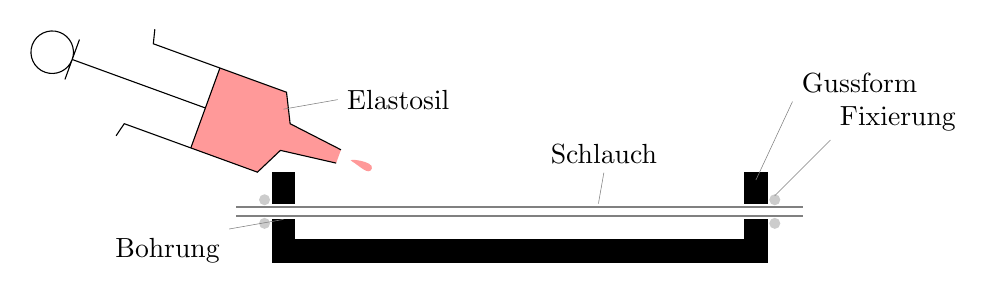
\begin{tikzpicture}[]


\draw [line width = 3mm] (-3,1)--(-3,.6) (-3,.4)--(-3,0)--(3,0)--(3,.4) (3,.6)--(3,1);

\draw [line width = .25mm, gray, double, double distance=1mm] (-3.6,.5)--(3.6,.5);

\fill [gray!40] (-3.24,.65) circle (.07) (-3.24,.35) circle (.07);
\fill [gray!40] (3.24,.65) circle (.07) (3.24,.35) circle (.07);


\begin{scope}[xshift=-2.3cm,yshift=1.2cm,rotate = 70, scale=.9]
\fill[red!40] (-.6,2)--(-.6,1)--(-.2,.8)--(-.1,0)--(.1,0)--(.2,.8)--(.6,1)--(.6,2);
\draw (-.8,3.05)--(-.6,3)--(-.6,1)--(-.2,.8)--(-.1,0);
\draw (.8,3.05)--(.6,3)--(.6,1)--(.2,.8)--(.1,0);
\draw (-.6,2)--(.6,2) (0,2)--(0,4) (-.3,4)--(.3,4) (0,4.3)circle(.3);
\fill[red!40] (0,-.2)to[out=260, in=180] (0,-.5) to [out=0, in = 85] (0,-.2);
\end{scope}


\draw[help lines] (3.24,.7)--++(45:1)node[above right, black]{Fixierung};
\draw[help lines] (3,.9)--++(65:1.1)node[above right, black]{Gussform};
\draw[help lines] (1,.6)--++(80:.4)node[above, black]{Schlauch};
\draw[help lines] (-3,.4)--++(190:.7)node[below left, black]{Bohrung};
\draw[help lines] (-3,1.8)--++(10:.7)node[right, black]{Elastosil};





\end{tikzpicture}
\end{document}